\chapter{Validation of the PACE Baseline}\label{ch:apdc}

\markboth{Appendix C}{}

Before running the main experimental campaign of this thesis, we validated our reimplementation of PACE against the results reported in the original paper by Thomas et al.~\cite{thomas_pace_2025}. The validation compares three configurations: PACE (with the bandit-based adoption mechanism), Greedy (which always adopts the shortest available program, eliminating the bandit), and No abstractions (which disables the Abstraction phase entirely). All three configurations are trained on the original uniform distribution (equivalent to $\alpha = 0.00$ in our parametrisation) and evaluated on the same 31-scene test set.

The validation focuses on two aggregate quantities that the original paper reports in its Figure 3: the mean program length across the 20 abstraction steps, and the reconstruction accuracy on the test set. Both curves are computed on the training set of 930 scenes and the held-out test set of 31 scenes.

\begin{figure}[htbp]
    \centering
    \IfFileExists{images/appendix_pace_validation_length.png}{%
        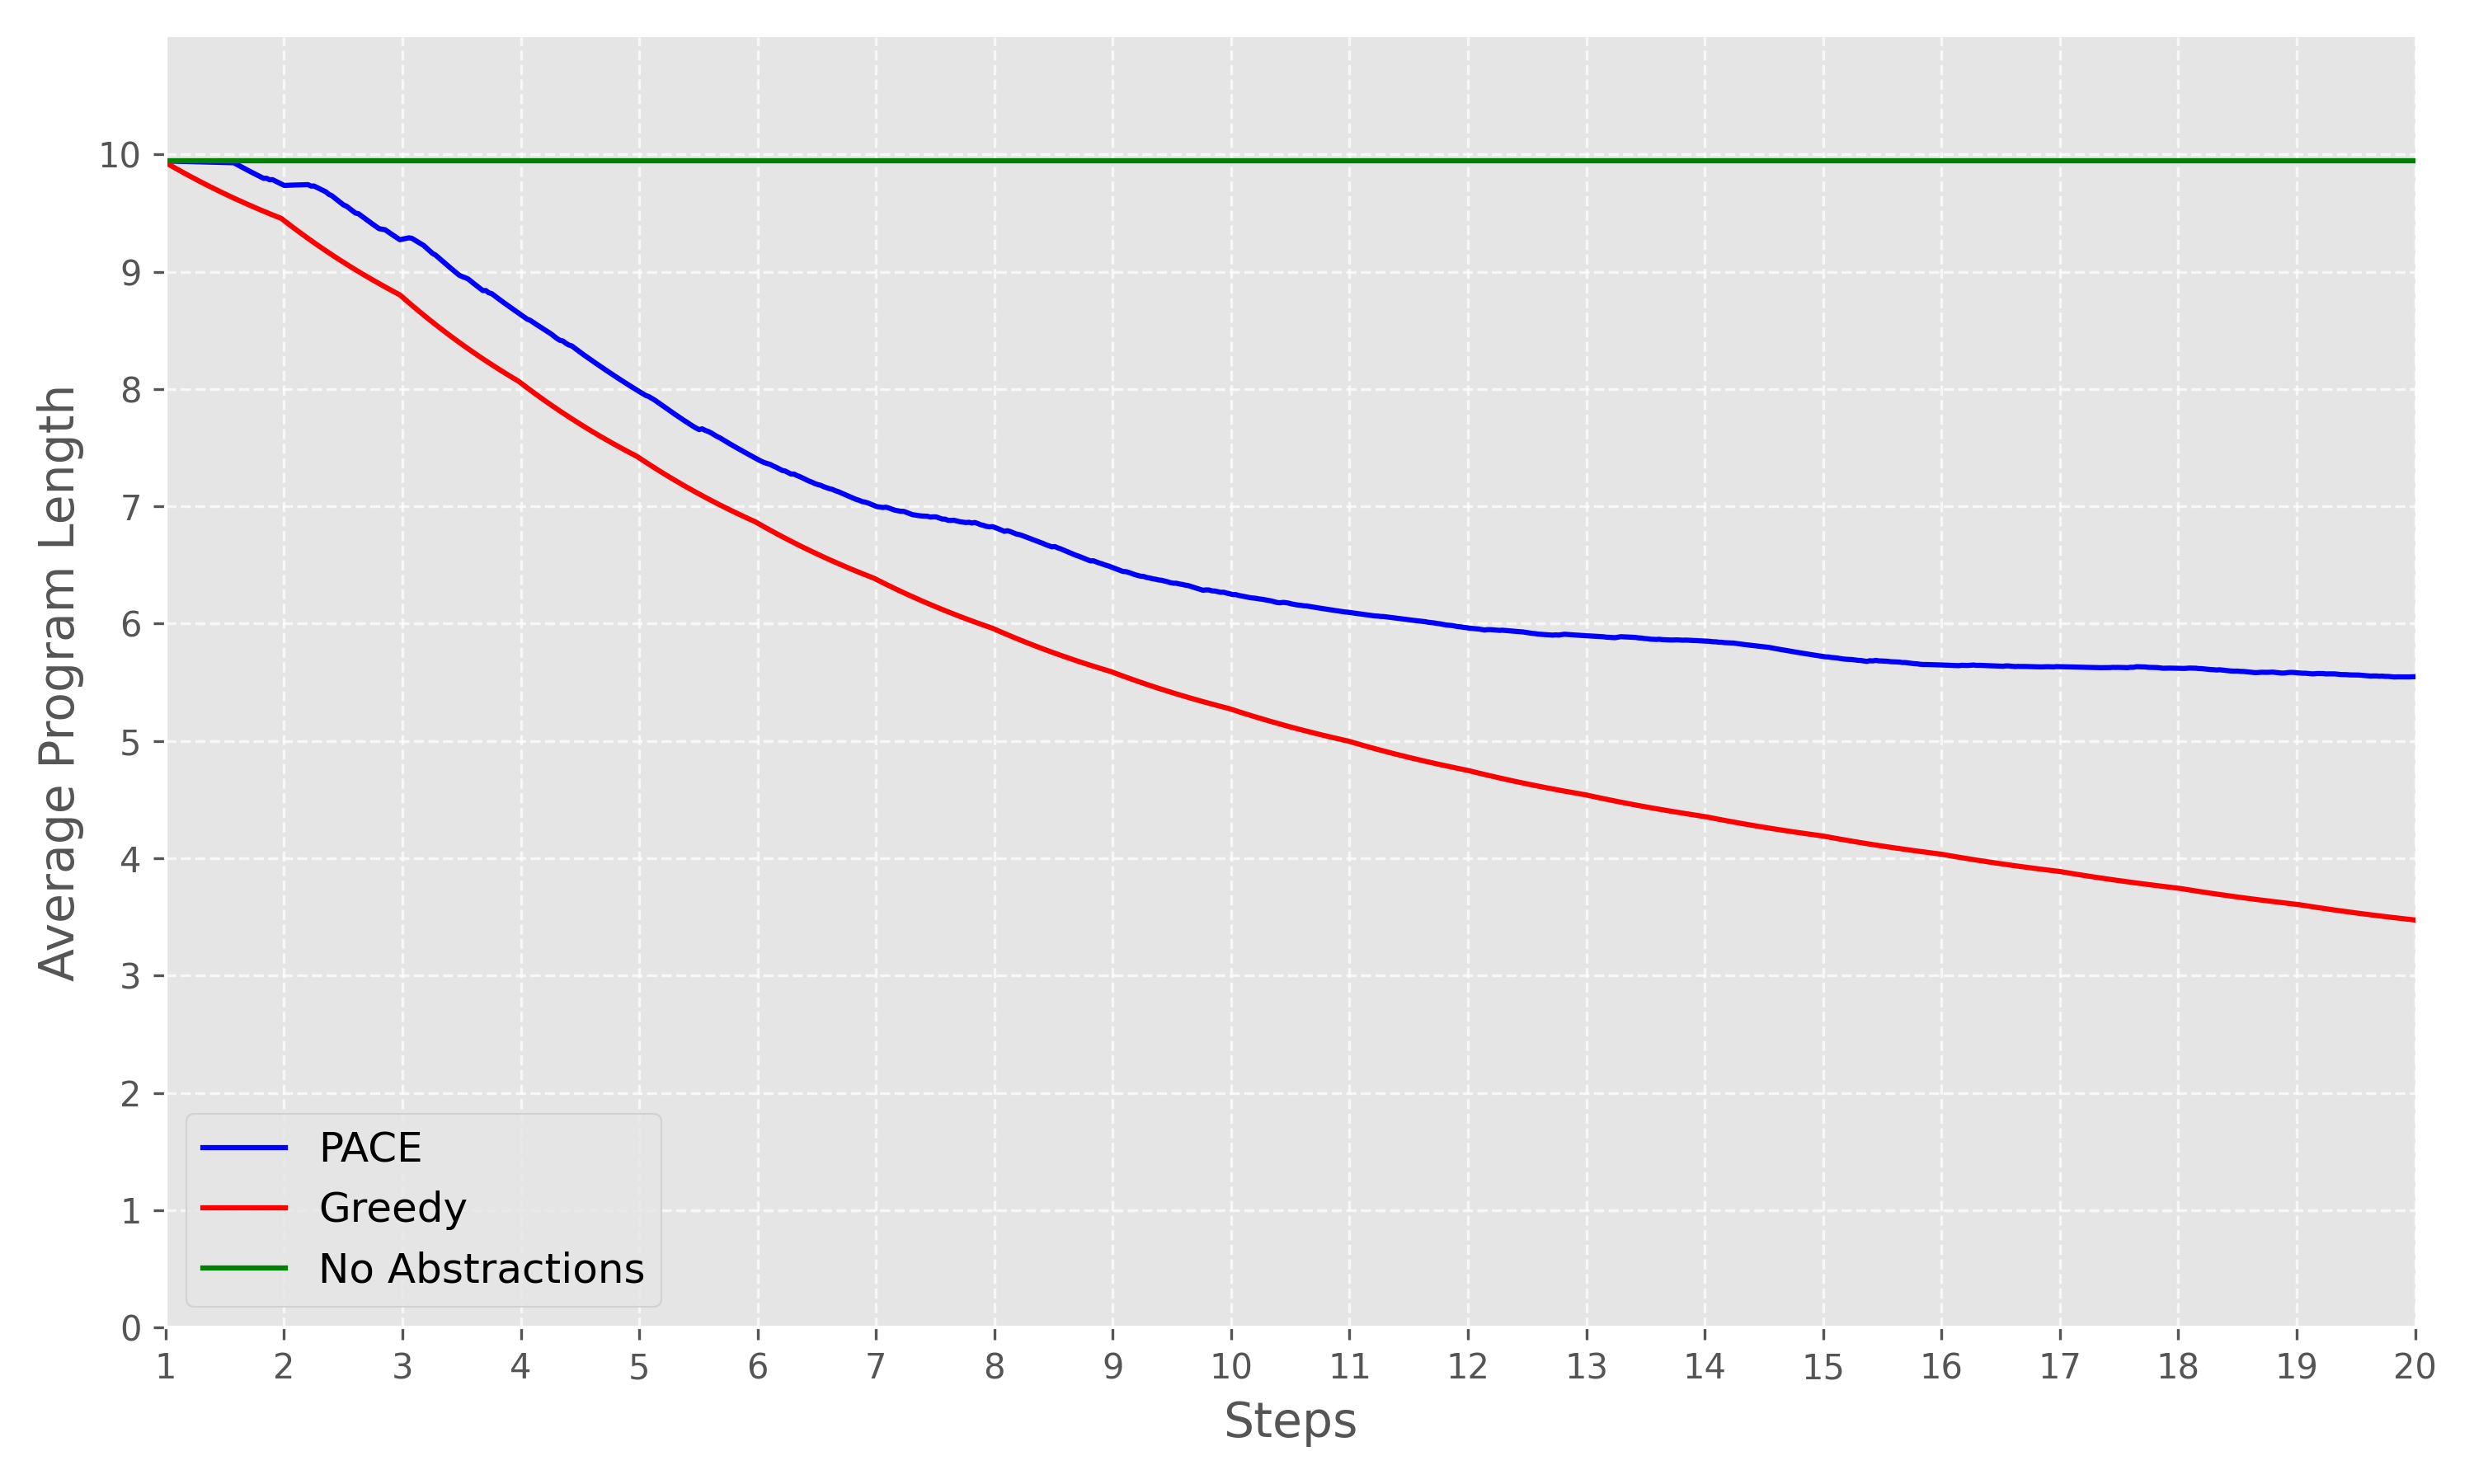
\includegraphics[width=0.95\textwidth]{images/appendix_pace_validation_length.png}%
    }{%
        \fcolorbox{red}{white}{\parbox[c][0.14\textheight][c]{0.9\textwidth}{\centering\textcolor{red}{Placeholder figure\\\texttt{\detokenize{images/appendix_pace_validation_length.png}}}}}%
    }
    \caption{Mean program length across the 20 abstraction steps for PACE, Greedy, and No abstractions. This replicates Figure 3 (left) of Thomas et al.~\cite{thomas_pace_2025}.}
    \label{fig:appendix-pace-validation-length}
\end{figure}

\begin{figure}[htbp]
    \centering
    \IfFileExists{images/appendix_pace_validation_accuracy.png}{%
        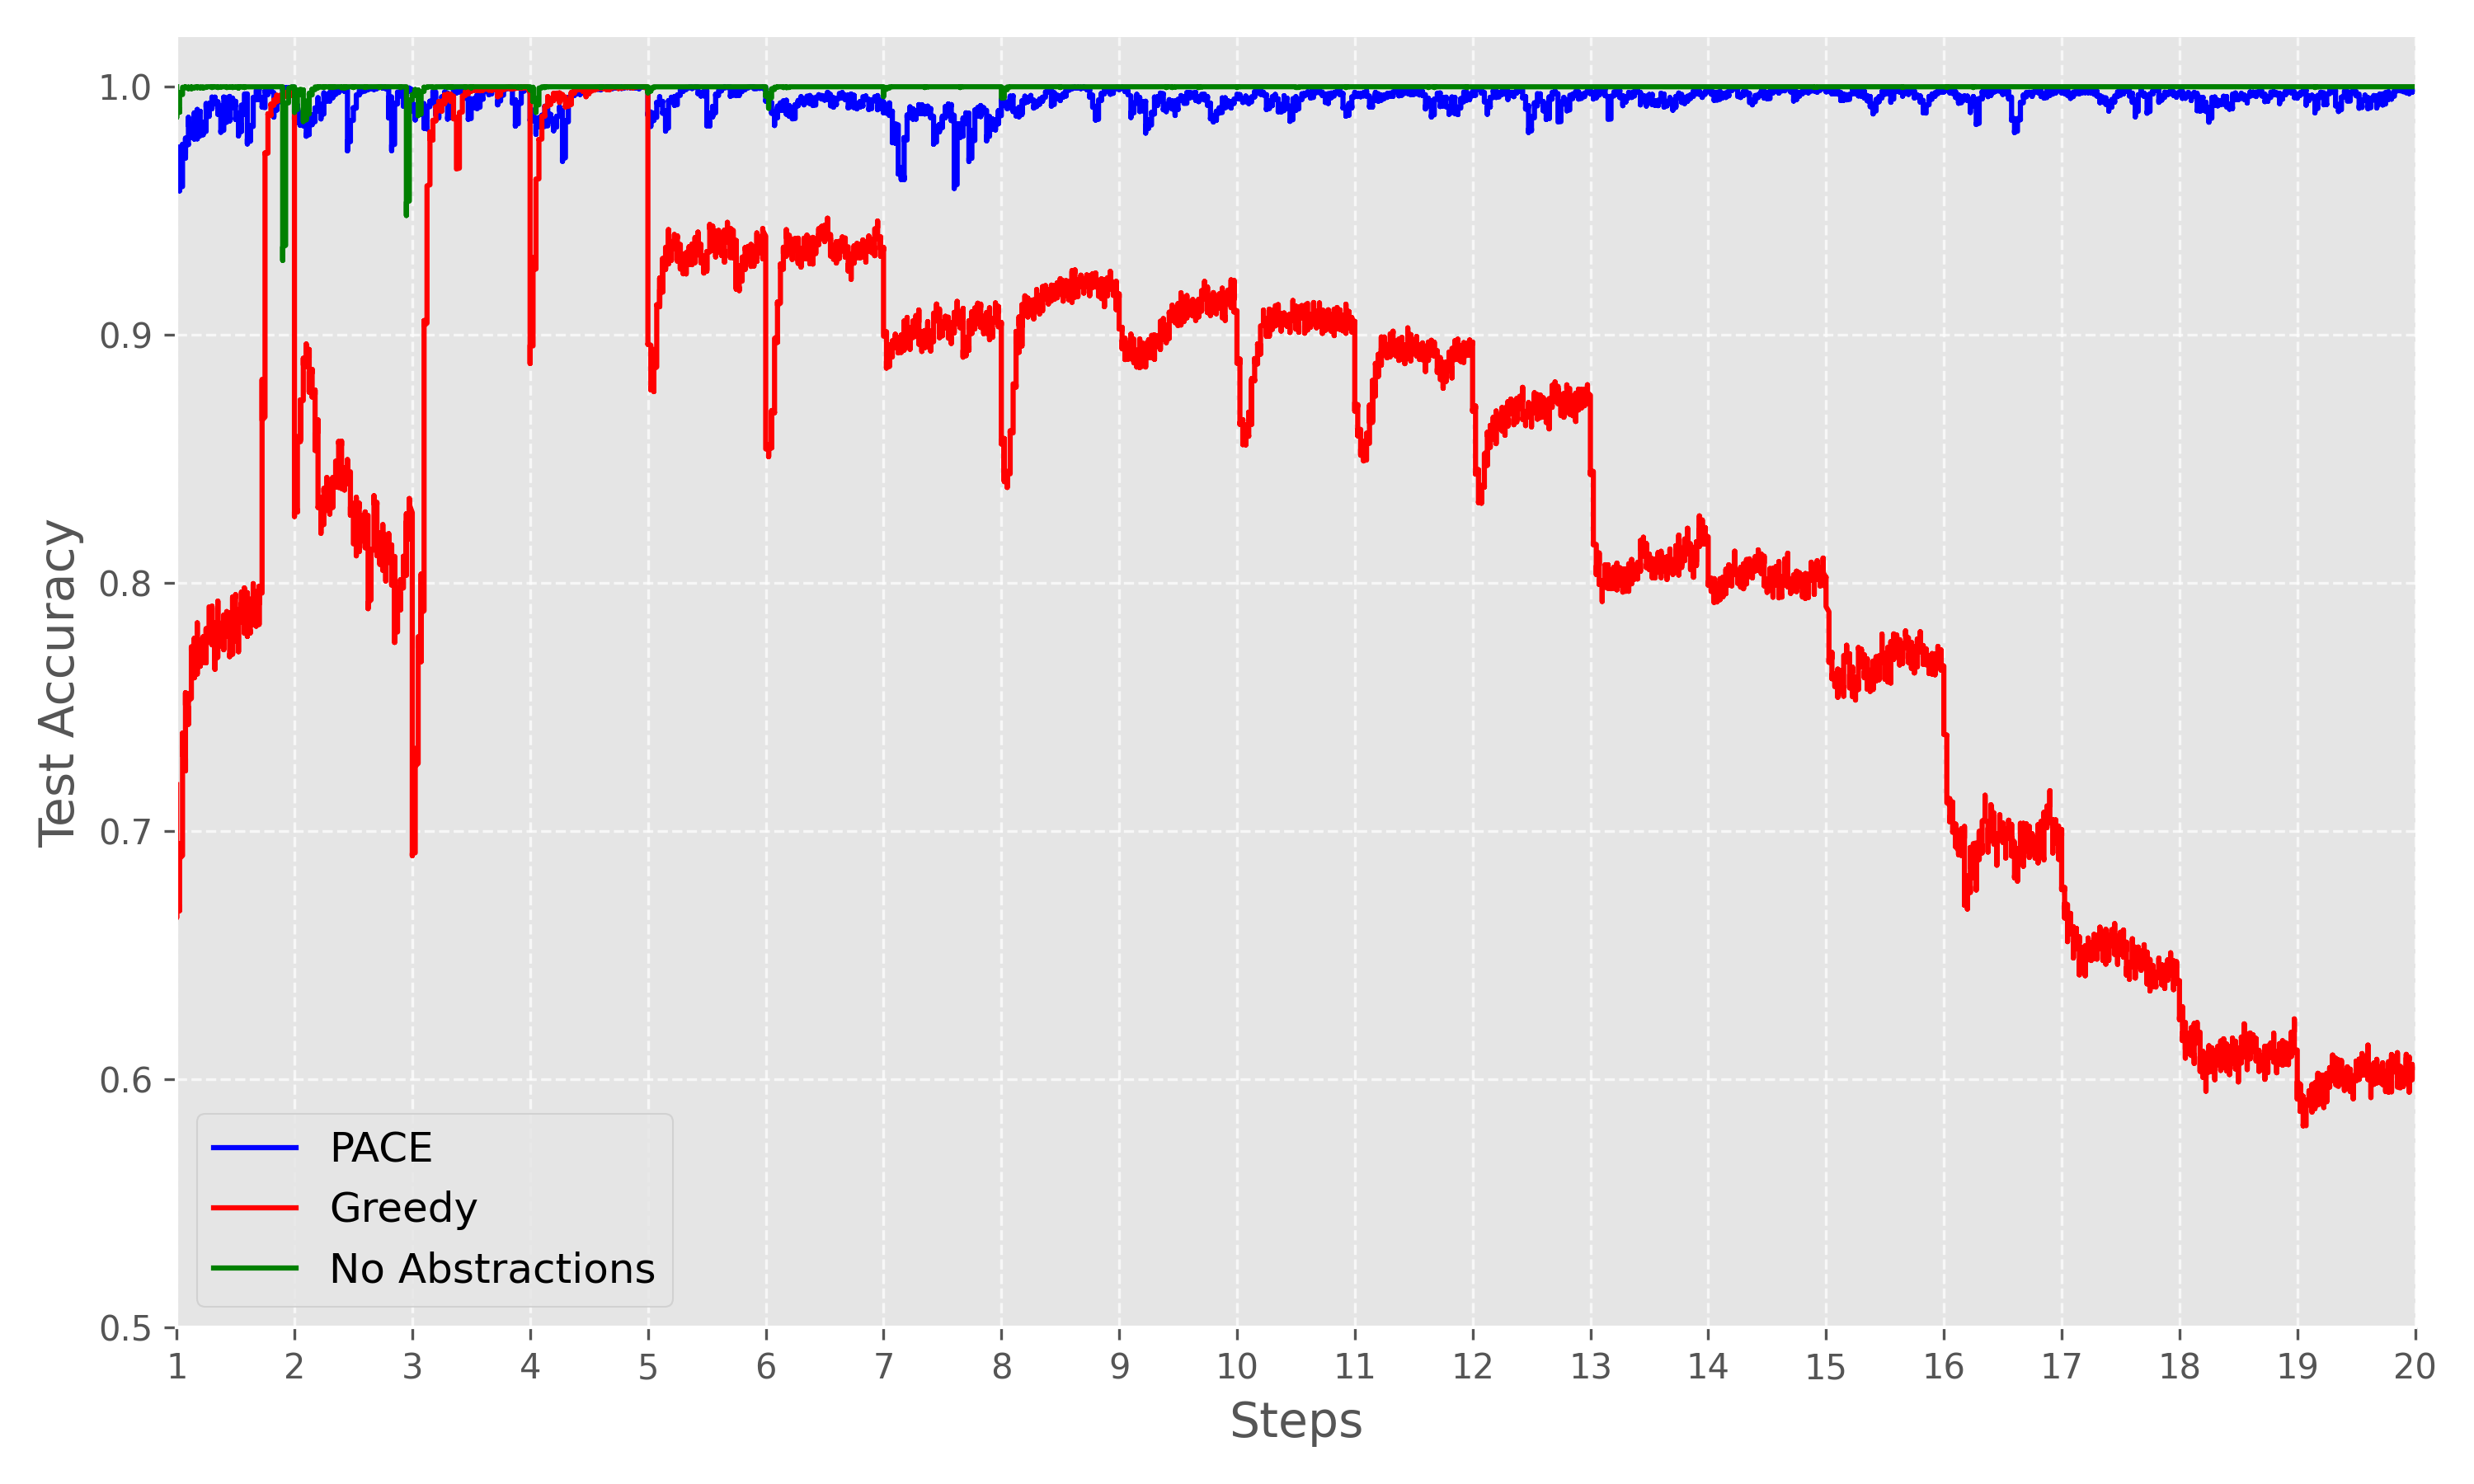
\includegraphics[width=0.95\textwidth]{images/appendix_pace_validation_accuracy.png}%
    }{%
        \fcolorbox{red}{white}{\parbox[c][0.14\textheight][c]{0.9\textwidth}{\centering\textcolor{red}{Placeholder figure\\\texttt{\detokenize{images/appendix_pace_validation_accuracy.png}}}}}%
    }
    \caption{Reconstruction accuracy on the test set across the 20 abstraction steps for PACE, Greedy, and No abstractions. This replicates Figure 3 (right) of Thomas et al.~\cite{thomas_pace_2025}.}
    \label{fig:appendix-pace-validation-accuracy}
\end{figure}

\section{Program Length Results}
\label{sec:appendix-program-length-results}

The three configurations produce clearly distinct compression trajectories, matching the qualitative behaviour reported in the original paper.

\begin{table}[htbp]
\centering
\begin{tabular}{lll}
\toprule
Configuration & Initial length (step 0) & Final length (step 19) \\
\midrule
No abstractions & 9.94 & 9.94 \\
Greedy & 9.94 & 3.20 \\
PACE & 9.94 & 5.33 \\
\bottomrule
\end{tabular}
\caption{Initial and final mean program length for the three validation configurations.}
\label{tab:appendix-program-length-results}
\end{table}

The No abstractions baseline shows no compression, as expected: without the Abstraction phase, the vocabulary consists only of the two primitives and no subsequences are ever replaced by shorter tokens. The Greedy variant compresses aggressively, reaching a final mean length of 3.20, while PACE compresses more moderately, converging to 5.33. This ordering matches the original paper's Figure 3 (left), where PACE settles around $4.92 \pm 0.20$ and Greedy compresses further.

Our final PACE length (5.33) differs from the $4.92 \pm 0.20$ reported in the paper, and we do not treat this as agreement within the seed-to-seed variability the paper reports across its 16 seeds. The convergence pattern, a rapid initial drop over the first several steps followed by a plateau, matches the shape of the original curve.

\section{Accuracy Results}
\label{sec:appendix-accuracy-results}

The three configurations also produce the expected accuracy behaviour.

\begin{table}[htbp]
\centering
\begin{tabular}{lll}
\toprule
Configuration & Final accuracy (step 19) & Mean accuracy across steps \\
\midrule
No abstractions & 1.00 & 1.00 \\
Greedy & 0.62 & 0.85 \\
PACE & 0.998 & 0.998 \\
\bottomrule
\end{tabular}
\caption{Final and mean reconstruction accuracy for the three validation configurations.}
\label{tab:appendix-accuracy-results}
\end{table}

The No abstractions baseline reaches perfect accuracy because it never introduces any new tokens: the neural agents only need to align on two primitives, and 40 epochs of joint training per step are sufficient. PACE maintains accuracy close to 1.00 throughout training, with a minimum of 0.989 across the 20 steps, because the bandit only adopts abstractions that the listener can interpret without disrupting communication. The Greedy variant, by contrast, shows the accuracy collapse that the original paper reports: forced to adopt new abstractions at every step regardless of interpretability, its accuracy drops progressively as training goes on, ending at 0.62.

This ordering, No abstractions $\approx$ PACE $>$ Greedy, matches Figure 3 (right) of Thomas et al.~\cite{thomas_pace_2025}, and shows that the trade-off between compression and interpretability is being handled by the bandit as intended.

\section{Number of Adopted Abstractions}
\label{sec:appendix-adopted-abstractions}

The number of abstractions adopted across the 20 steps is also consistent with the original paper.

\begin{table}[htbp]
\centering
\begin{tabular}{ll}
\toprule
Configuration & Adopted abstractions \\
\midrule
No abstractions & 0 \\
Greedy & 18 \\
PACE & 6 \\
\bottomrule
\end{tabular}
\caption{Number of abstractions adopted by each validation configuration.}
\label{tab:appendix-adopted-abstractions}
\end{table}

The No abstractions baseline never enters the Abstraction phase and adopts no abstractions. PACE adopts 6 abstractions across the 20 steps, converging on a stable vocabulary well before the 20th step, in line with the paper's observation that PACE naturally stops introducing new abstractions once the language is sufficiently developed. Greedy adopts 18 abstractions, matching its aggressive adoption behaviour.

\section{Summary}
\label{sec:appendix-validation-summary}

The three configurations reproduce the qualitative behaviour of Figure 3 in Thomas et al.~\cite{thomas_pace_2025}: the No abstractions baseline reaches perfect accuracy at no compression, the Greedy variant compresses aggressively but loses accuracy, and PACE achieves the intended balance between the two. The final PACE program length is 5.33, compared with the reported $4.92 \pm 0.20$, a difference of 0.41. This comparison supports qualitative rather than exact numerical agreement; it does not establish that the discrepancy falls within the seed-to-seed variability reported in the paper. On this basis, we proceed to the main experimental campaign of the thesis, which extends PACE from a uniform training distribution to the Zipfian family described in Chapters~\ref{ch:pace} and~\ref{ch:technical}.